% Security evaluation figure, experiment 15. Just the float.
%
% Needs: figures/sec-grid.pdf, from
%   paper_experiments/15-security-evaluation/figures/sec-grid.pdf
% regenerated by gem5-DIT/benchmarks/expedite_security/plot_paper_figs.py
% from that experiment's data/results.csv.
%
% figure* spans both columns. figures/sec-grid-col.pdf is the same four
% panels laid out for a single-column figure, and the panels also exist
% standalone as figures/sec-{vp,dmp,compsimp,spec}.pdf.
%
% Self-contained: no siunitx, and no \ref out to surrounding text.

\begin{figure*}[t]
  \centering
  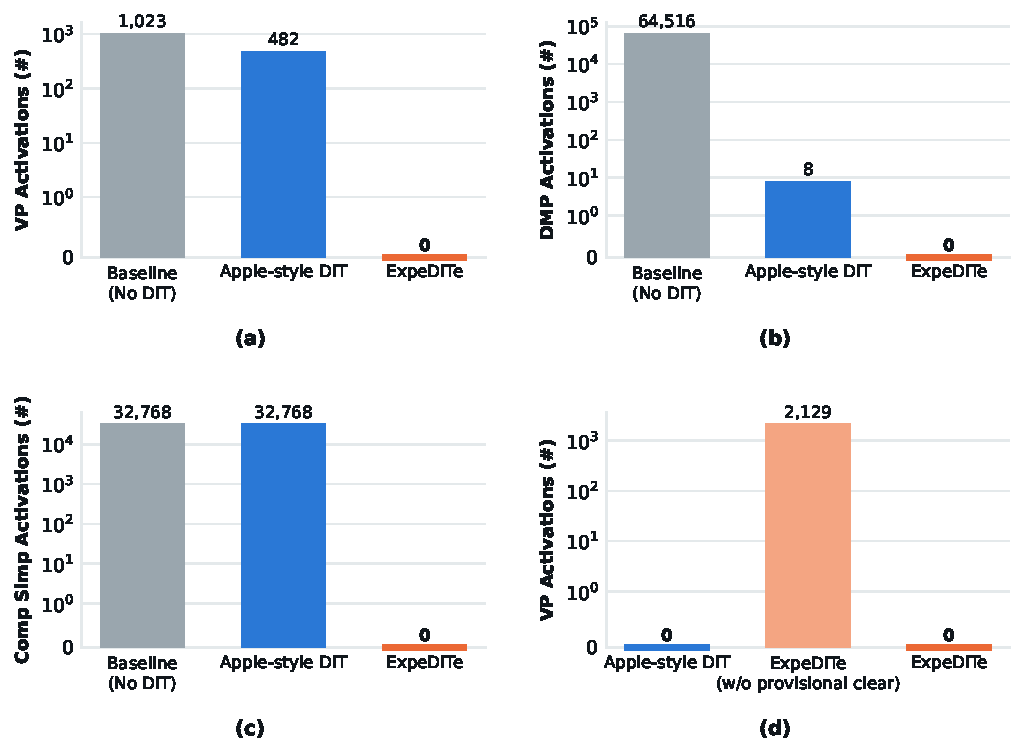
\includegraphics[width=\textwidth]{figures/sec-grid.pdf}
  \caption{Each gated optimization acting inside the DIT region. (a)~activations
  of the value predictor on the secret loads, net of the training loads the
  probe predicts outside any region; (b)~DMP activations, each one a prefetch
  of a line addressed by a secret pointer; (c)~computation simplifications,
  that is multiplies that ran with operand-dependent latency, of the 32{,}768
  in the region. In (a)--(c) the baseline is the same binary
  with the mode switches removed, and \emph{Apple-style DIT} is the gem5 model
  of Apple's design (\texttt{-{}-apple}): the switch is unordered against older
  instructions and establishes the mode only when it commits. Every
  optimization activates on the baseline and under Apple-style DIT, and none
  activates under ExpeDITe. (d)~value-predictor activations on loads that were
  architecturally \emph{inside} the DIT region and executed only
  speculatively, behind a clear that never architecturally executed: loads that
  should have been gated. Apple-style DIT reads zero here for a structural
  reason rather than as a defence: it establishes the mode only when the write
  commits, so a clear on a wrong path never takes effect and the case does not
  arise for it -- the same property that makes it leak at region entry
  in~(a)--(c). \emph{ExpeDITe (w/o provisional clear)} is the identical
  ExpeDITe binary with its deferred clear published as soon as it executes.}
  \label{fig:sec-grid}
\end{figure*}
